\documentclass[12pt]{article}

\usepackage[margin=2cm]{geometry}
\usepackage[T2A]{fontenc}
\usepackage[utf8]{inputenc}
\usepackage[russian]{babel}
\usepackage{multicol}
\usepackage{longtable}
\usepackage{graphics}
\usepackage{rotating}
\usepackage{float}
\usepackage{indentfirst}

\setlength{\parindent}{2em}
\setlength{\parskip}{1em}

\usepackage{amsmath, amsfonts, amssymb, amsthm, mathtools}
\usepackage{icomma}

\title{Отчет о выполнении лабораторной работы \\ Исследование взаимной диффузии газов}
\author{Лепарский Роман}
\date{\today}

\begin{document}

\maketitle

\newpage

\section{Аннотация}

\textbf{Цель работы:} 1) регистрация зависимости концентрации гелия в воздухе от времени с помощью датчиков теплопроводности
при разных начальных давлениях смеси газов; 2) определение 
коэффициента диффузии по результатам измерений.

\section{Теоретические сведения}

Диффузией называется самопроизвольное перемешивание молекул, происходящее вследствие их хаотического теплового движения.

Плотность потока вещества в результате взаимной диффузии определяется законом Фика:
\begin{equation}
	j = -D\frac{\partial n}{\partial x}
\end{equation}

Поскольку объем трубки много меньше объемов сосудов, 
концентрацию в последних можно считать постоянной. Пусть в объемах $V_1$ и $V_2$ поддерживаются постоянные концентрации
$n_1$ и $n_2$. Тогда в трубе установится постоянный поток $J = -DS\frac{\partial n}{\partial x}$. Отсюда $n(x)$ - линейная функция. Если подставить длину трубки $l$, получим:
\begin{equation}
	J = -DS\frac{n_1 - n_2}{l}
\end{equation}

Изменение компонента в сосудах: $V_1\Delta n_1=-V_2\Delta n_2$

С другой стороны $V_1\Delta n_1=-V_2\Delta n_2=J\Delta t$

Разделив на $\Delta t$ получим:
\[
	V_1\frac{dn_1}{dt}=-V_2\frac{dn_2}{dt}=-DS\frac{n_1-n_2}{l}
\]
После преобразований получим:
\[
	\frac{dn_1}{dt} - \frac{dn_2}{dt} = -\frac{n_1-n_2}{l}DS\left(\frac{1}{V_1} + \frac{1}{V_2}\right)
\]
Примем $\Delta n = n_1 - n_2$, $\Delta n_0$ - разность концентраций примеси в начальный момент времени:
\begin{equation}
	\Delta n=\Delta n_0 e^{-t/\tau},  \tau=\frac{V_1V_2}{V_1+V_2}\frac{l}{SD}
	\label{eq:tauIs}
\end{equation}

Напряжение на мосту убывает по экспоненциальному закону с тем же показателем. Прологарифмировав получим:
\begin{equation}
	\ln{V} = \ln{V_0} - \frac{t}{\tau}
	\label{eq:main}
\end{equation} 

\section{Экспериментальная установка}

\begin{figure}[H]
	\centering
	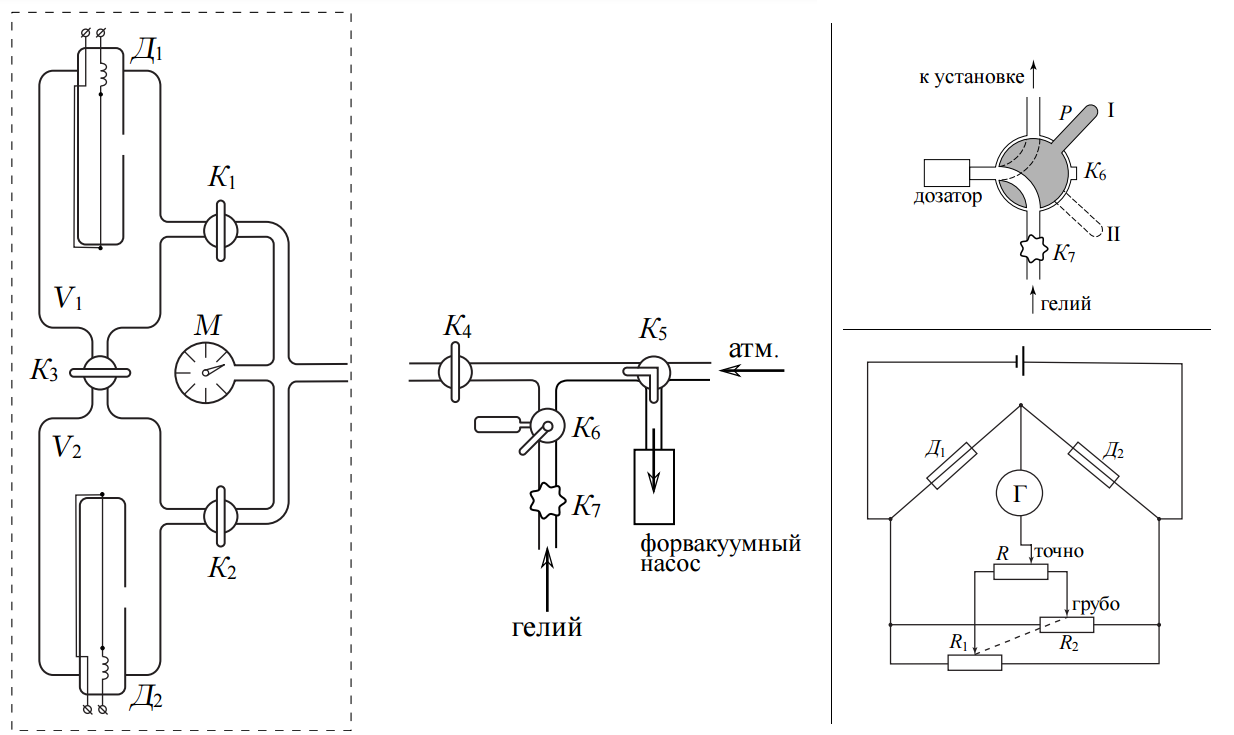
\includegraphics[scale = 0.5]{./images/stand.png}
	\caption{Схема установки}
	\label{fig:stand}
\end{figure}
Для исследования взаимной диффузии газов  и определения коэффициента диффузии используется установка, изображенная на рис.\ref{fig:stand}. Два сосуда соединены трубкой сечения $S$ и  длины $l$. Сосуды заполнены смесью газов при одинаковом давлении.

\section{Приборы и материалы}

В работе используются:

\begin{itemize}
	\item Измерительная установка;
	\item Форвакуумный насос;
	\item манометр;
	\item Баллон с газом (гелий);
	\item Источник питания;
	\item Магазин сопротивлений;
	\item Гальванометр;
	\item Секундомер.
\end{itemize}

\section{Обработка результатов}

Проведем измерения при различных давлениях. Таблицы с измеренными значениями находятся в приложении.
По этим значениям построим графики и найдем коэффициент наклона $1/\tau$

\begin{figure}[H]
	\centering
	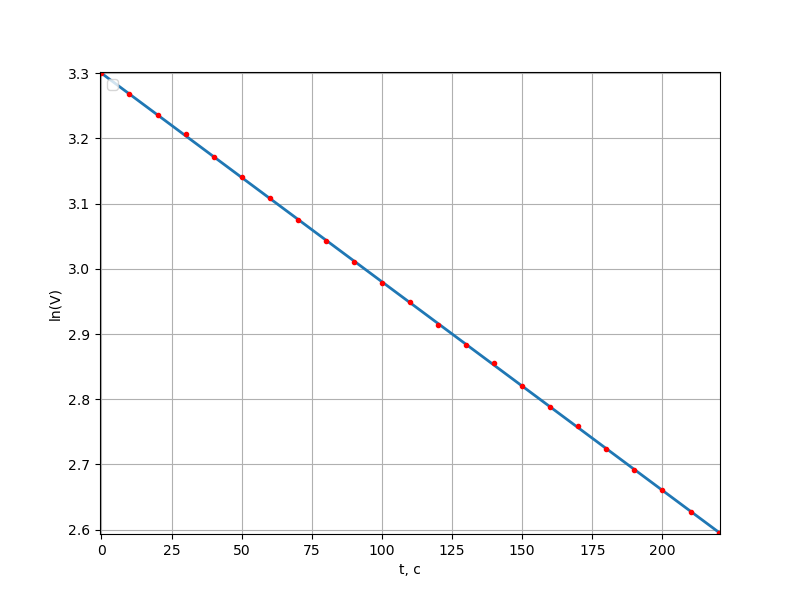
\includegraphics[scale = 0.695]{./images/Gr1.png}
	\caption{$P_\text{раб} = 47,8$ Торр;  $1/\tau = (3200 \pm 4) \cdot 10^{-6}$ c$^{-1}$}
	\label{fig:Gr1}
\end{figure}

\begin{figure}[H]
	\centering
	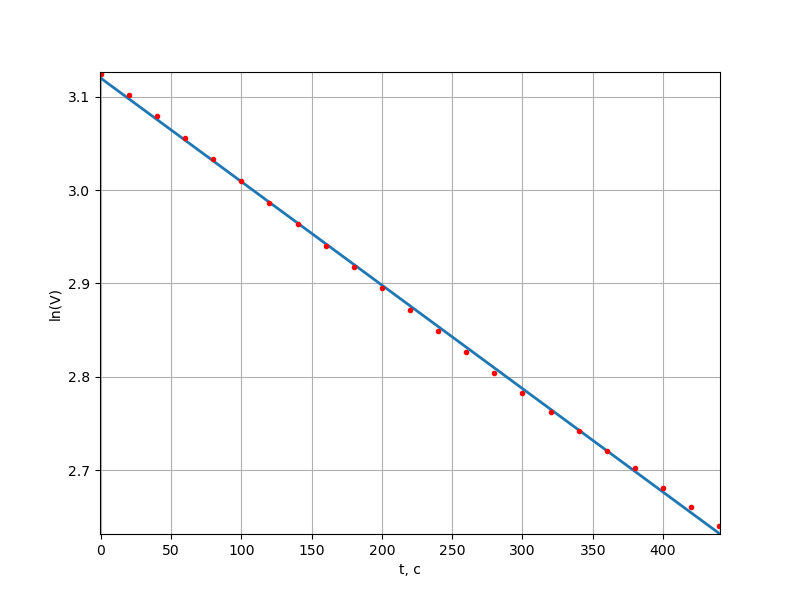
\includegraphics[scale = 0.695]{./images/Gr2.png}
	\caption{$P_\text{раб} = 117,6$ Торр;  $1/\tau = (1108 \pm 6) \cdot 10^{-6}$ c$^{-1}$}
	\label{fig:Gr2}
\end{figure}

\begin{figure}[H]
	\centering
	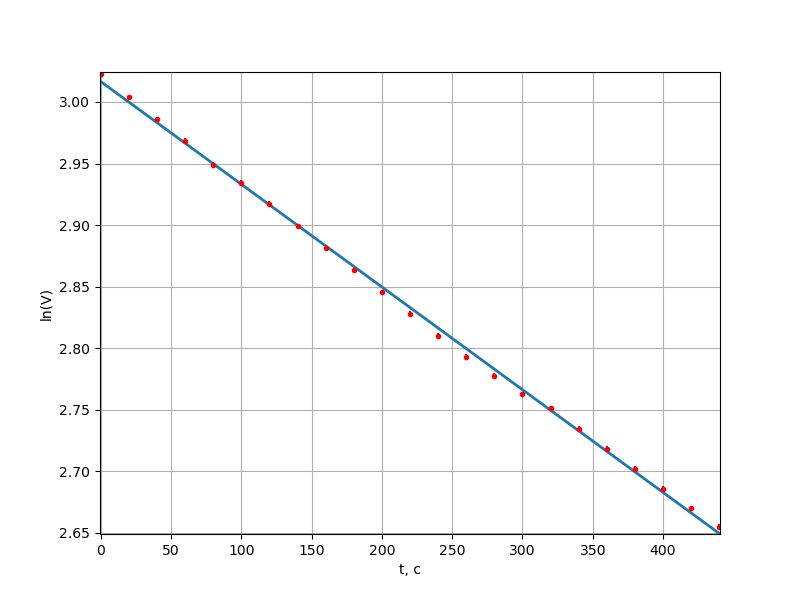
\includegraphics[scale = 0.695]{./images/Gr3.png}
	\caption{$P_\text{раб} = 183,8$ Торр;  $1/\tau = (834 \pm 5) \cdot 10^{-6}$ c$^{-1}$}
	\label{fig:Gr3}
\end{figure}

\begin{figure}[H]
	\centering
	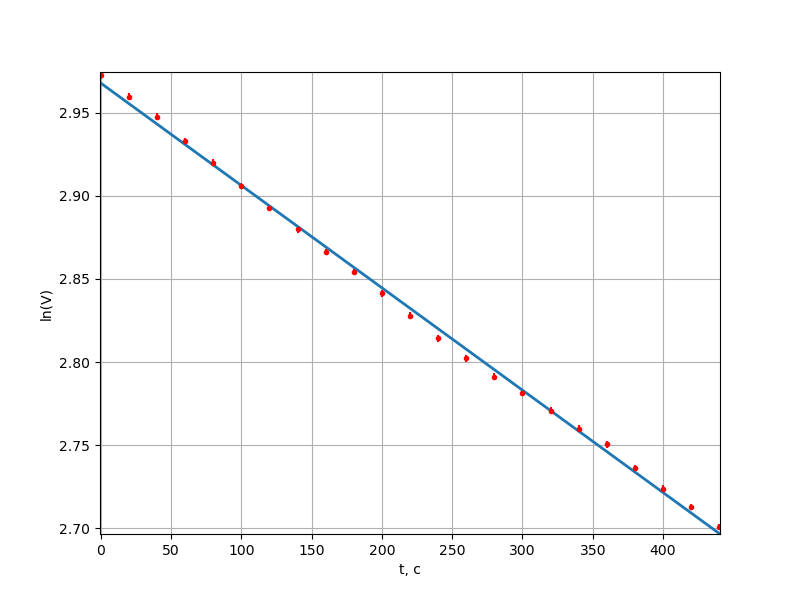
\includegraphics[scale = 0.695]{./images/Gr4.png}
	\caption{$P_\text{раб} = 241,1$ Торр;  $1/\tau = (615 \pm 5) \cdot 10^{-6}$ c$^{-1}$}
	\label{fig:Gr4}
\end{figure}

\begin{figure}[H]
	\centering
	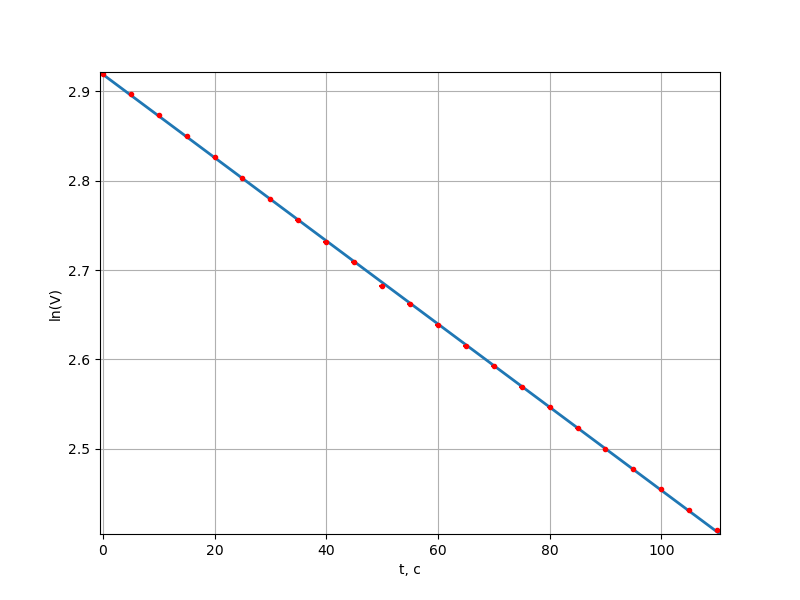
\includegraphics[scale = 0.695]{./images/Gr5.png}
	\caption{$P_\text{раб} = 22,1$ Торр;  $1/\tau = (4651 \pm 8) \cdot 10^{-6}$ c$^{-1}$}
	\label{fig:Gr5}
\end{figure}

На последнем графике и в таблице 6 соответственно представлена зависимость концентрации гелия от времени, но при проникновении смеси воздух-гелий в чистый гелий, чтобы показать, что это не влияет на итоговый результат.

Запишем в таблицу значения коэффициента $1/\tau$ и найдем по ним коэффициент диффузии из формулы (\ref{eq:tauIs}). Так же внесем таблицу величину $1/P$:

\begin{table}[H]
	\centering
	\begin{tabular}{|l|l|l|l|}
		\hline
		N & $1/P$, Torr$^{-1}$ & $1/\tau$, $10^{-6}$ 1/c & $D$, см$^2$/с \\ \hline
		1 & 0,02092050209205   & 3200                    & 11,9         \\ \hline
		2 & 0,008503401360544  & 1108                    & 4,1         \\ \hline
		3 & 0,00544069640914   & 834                     & 3,1        \\ \hline
		4 & 0,004147656574036  & 615                     & 2,3        \\ \hline
		5 & 0,045248868778281  & 4651                    & 17,4       \\ \hline
	\end{tabular}
\end{table}

Рассчитаем приблизительно погрешность $D$. Примем $V_1 = V_2 = V$.
\begin{equation*}
	\sigma_D^2 = \left(\frac{l}{2S\tau}\right)^2\sigma_V^2 + \left(\frac{V}{2\tau}\right)^2\sigma_{l/s}^2 + \left(\frac{Vl}{2S}\right)^2\sigma_{1/\tau}^2
\end{equation*}

Отсюда $\sigma_D = 0,2$ см$^2$/с.

Построим график зависимости $D(1/P)$ по данным значениям.

\begin{figure}[H]
	\centering
	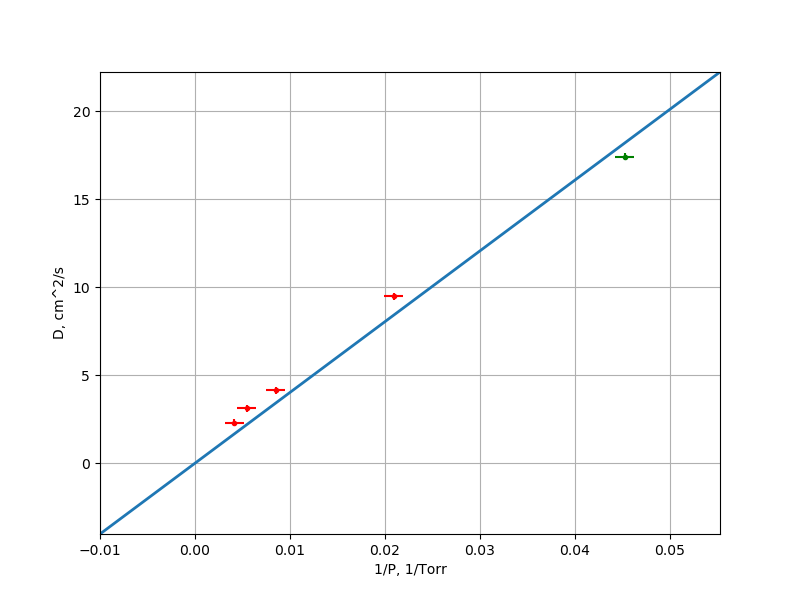
\includegraphics[scale = 0.695]{./images/Gr6.png}
	\label{fig:Gr6}
\end{figure}

Рассчитав по данной прямой значение для атмосферного давления (735 mmHg) получим $D_\text{атм} = 0,56 \pm 0,03$ см$^2$/с.

Оценим длину свободного пробега молекулы и ее диаметр:

\begin{equation*}
	\lambda = \frac{3D}{\left<V\right>} \thicksim 1.3 \cdot 10^{-7} \text{ м}
\end{equation*}

\begin{equation*}
	d = \sqrt{\frac{kT}{\pi P \lambda}} \thicksim 0.26 \text{ нм}
\end{equation*}

\section{Вывод}

Посчитав коэффициент диффузии для нескольких точек, мы смогли приблизительно найти коэффициент диффузии гелия в воздухе при атмосферном давлении $D_\text{атм} = 0,56 \pm 0,03$ см$^2$/с. Что лежит довольно близко к табличному значению (0,62 см$^2$/с). С помощью одного дополнительного измерения можно увидеть, что этот коэффициент не зависит от начальной концентрации гелия в воздухе. Также получилось оценить длину пробега $\lambda \thicksim 1.3 \cdot 10^{-7} \text{ м}$ и диаметр молекулы гелия $d \thicksim 0.26 \text{ нм}$. Эти значения тоже близки к табличным \newline($\lambda = 1.75 \cdot 10^{-7} \text{ м}$, $d = 0.20 \text{ нм}$).

\newpage
\section*{Приложение}

\begin{table}[H]
	\centering
	\begin{tabular}{|l|l|l|}
		\hline
		t, c & V, mv & ln(V)            \\ \hline
		0    & 27,11 & 3,29990266351057 \\ \hline
		10   & 26,26 & 3,26804686887465 \\ \hline
		20   & 25,44 & 3,23632273847192 \\ \hline
		30   & 24,69 & 3,20639830335709 \\ \hline
		40   & 23,86 & 3,17220341666977 \\ \hline
		50   & 23,11 & 3,14026542428629 \\ \hline
		60   & 22,38 & 3,10816770288378 \\ \hline
		70   & 21,66 & 3,07546724157284 \\ \hline
		80   & 20,97 & 3,04309284491383 \\ \hline
		90   & 20,29 & 3,01012815383772 \\ \hline
		100  & 19,64 & 2,97756830292632 \\ \hline
		110  & 19,09 & 2,94916463773766 \\ \hline
		120  & 18,44 & 2,91452221812845 \\ \hline
		130  & 17,88 & 2,88368276974537 \\ \hline
		140  & 17,39 & 2,85589532836619 \\ \hline
		150  & 16,78 & 2,82018770103906 \\ \hline
		160  & 16,25 & 2,78809290877575 \\ \hline
		170  & 15,78 & 2,75874331541773 \\ \hline
		180  & 15,24 & 2,7239235502585  \\ \hline
		190  & 14,76 & 2,69192081917233 \\ \hline
		200  & 14,3  & 2,66025953726586 \\ \hline
		210  & 13,84 & 2,62756295018952 \\ \hline
		220  & 13,4  & 2,59525470695687 \\ \hline
	\end{tabular}
	\caption{$P_\text{раб} = 47,8$ Торр}
\end{table}

\begin{table}[H]
	\centering
	\begin{tabular}{|l|l|l|}
		\hline
		t, c & V, mv & ln(V)            \\ \hline
		0    & 22,75 & 3,12456514539696 \\ \hline
		20   & 22,24 & 3,10189246938238 \\ \hline
		40   & 21,75 & 3,07961375753469 \\ \hline
		60   & 21,25 & 3,05635689537043 \\ \hline
		80   & 20,76 & 3,03302805829769 \\ \hline
		100  & 20,28 & 3,00963517872298 \\ \hline
		120  & 19,81 & 2,98618686071046 \\ \hline
		140  & 19,36 & 2,96320908184843 \\ \hline
		160  & 18,92 & 2,94021956362373 \\ \hline
		180  & 18,5  & 2,91777073208428 \\ \hline
		200  & 18,09 & 2,8953592994072  \\ \hline
		220  & 17,67 & 2,87186828633161 \\ \hline
		240  & 17,27 & 2,84897089215859 \\ \hline
		260  & 16,88 & 2,82612948916781 \\ \hline
		280  & 16,51 & 2,80396625793204 \\ \hline
		300  & 16,17 & 2,78315767358902 \\ \hline
		320  & 15,84 & 2,76253838638628 \\ \hline
		340  & 15,51 & 2,74148497718845 \\ \hline
		360  & 15,18 & 2,71997877196748 \\ \hline
		380  & 14,92 & 2,70270259477561 \\ \hline
		400  & 14,6  & 2,68102152871429 \\ \hline
		420  & 14,3  & 2,66025953726586 \\ \hline
		440  & 14,01 & 2,63977136034892 \\ \hline
	\end{tabular}
	\caption{$P_\text{раб} = 117,6$ Торр}
\end{table}

\begin{table}[H]
	\centering
	\begin{tabular}{|l|l|l|}
		\hline
		t, c & V, mv & ln(V)            \\ \hline
		0    & 20,54 & 3,02237420450041 \\ \hline
		20   & 20,16 & 3,00370044320317 \\ \hline
		40   & 19,81 & 2,98618686071046 \\ \hline
		60   & 19,46 & 2,96836107675786 \\ \hline
		80   & 19,09 & 2,94916463773766 \\ \hline
		100  & 18,81 & 2,93438864331294 \\ \hline
		120  & 18,49 & 2,91723004539903 \\ \hline
		140  & 18,16 & 2,89922137317315 \\ \hline
		160  & 17,84 & 2,88144312715186 \\ \hline
		180  & 17,52 & 2,86334308550825 \\ \hline
		200  & 17,21 & 2,84549061022345 \\ \hline
		220  & 16,91 & 2,82790516291049 \\ \hline
		240  & 16,61 & 2,8100049236252  \\ \hline
		260  & 16,33 & 2,79300390698237 \\ \hline
		280  & 16,08 & 2,77757626375082 \\ \hline
		300  & 15,84 & 2,76253838638628 \\ \hline
		320  & 15,66 & 2,75110969056266 \\ \hline
		340  & 15,4  & 2,73436750941958 \\ \hline
		360  & 15,15 & 2,71800053195538 \\ \hline
		380  & 14,91 & 2,70203212877665 \\ \hline
		400  & 14,67 & 2,68580459215489 \\ \hline
		420  & 14,44 & 2,67000213346468 \\ \hline
		440  & 14,22 & 2,65464942437509 \\ \hline
	\end{tabular}
	\caption{$P_\text{раб} = 183,8$ Торр}
\end{table}

\begin{table}[H]
	\centering
	\begin{tabular}{|l|l|l|}
		\hline
		t, c & V, mv & ln(V)            \\ \hline
		0    & 19,54 & 2,97246364661464 \\ \hline
		20   & 19,29 & 2,95958682691764 \\ \hline
		40   & 19,06 & 2,94759189822606 \\ \hline
		60   & 18,78 & 2,93279247378012 \\ \hline
		80   & 18,54 & 2,91993056013771 \\ \hline
		100  & 18,28 & 2,905807566026   \\ \hline
		120  & 18,04 & 2,89259151463448 \\ \hline
		140  & 17,81 & 2,87976009730157 \\ \hline
		160  & 17,57 & 2,86619290219901 \\ \hline
		180  & 17,36 & 2,8541687092322  \\ \hline
		200  & 17,14 & 2,84141491316963 \\ \hline
		220  & 16,91 & 2,82790516291049 \\ \hline
		240  & 16,68 & 2,8142103969306  \\ \hline
		260  & 16,48 & 2,80214752448133 \\ \hline
		280  & 16,3  & 2,79116510781272 \\ \hline
		300  & 16,14 & 2,7813006628418  \\ \hline
		320  & 15,97 & 2,77071196222692 \\ \hline
		340  & 15,8  & 2,76000994003292 \\ \hline
		360  & 15,65 & 2,75047091698616 \\ \hline
		380  & 15,43 & 2,73631366637507 \\ \hline
		400  & 15,24 & 2,7239235502585  \\ \hline
		420  & 15,07 & 2,7127060126384  \\ \hline
		440  & 14,89 & 2,70068984669592 \\ \hline
	\end{tabular}
	\caption{$P_\text{раб} = 241,1$ Торр}
\end{table}

\begin{table}[H]
	\centering
	\begin{tabular}{|l|l|l|}
		\hline
		t, c & V, mv & ln(V)            \\ \hline
		0    & 18,53 & 2,91939104029727 \\ \hline
		5    & 18,12 & 2,89701630061483 \\ \hline
		10   & 17,7  & 2,87356463957978 \\ \hline
		15   & 17,29 & 2,8501282996952  \\ \hline
		20   & 16,89 & 2,82672173081971 \\ \hline
		25   & 16,5  & 2,80336038090653 \\ \hline
		30   & 16,11 & 2,77944019718888 \\ \hline
		35   & 15,73 & 2,75556971707019 \\ \hline
		40   & 15,35 & 2,73111547403321 \\ \hline
		45   & 15,01 & 2,70871664564537 \\ \hline
		50   & 14,62 & 2,68239045432163 \\ \hline
		55   & 14,33 & 2,66235524184008 \\ \hline
		60   & 13,99 & 2,63834278867739 \\ \hline
		65   & 13,67 & 2,61520365073586 \\ \hline
		70   & 13,36 & 2,5922651681085  \\ \hline
		75   & 13,05 & 2,5687881337687  \\ \hline
		80   & 12,76 & 2,54631527791664 \\ \hline
		85   & 12,47 & 2,52332575969195 \\ \hline
		90   & 12,18 & 2,49979526228175 \\ \hline
		95   & 11,91 & 2,47737838336721 \\ \hline
		100  & 11,65 & 2,45530618001171 \\ \hline
		105  & 11,38 & 2,43185742869818 \\ \hline
		110  & 11,13 & 2,40964416528745 \\ \hline
	\end{tabular}
	\caption{$P_\text{раб} = 22,1$ Торр}
\end{table}

\end{document}